\label{sec:single_crystal_section}
  Постепенно будем наполнять схему и внесем один идеальный кристаллический элемент.
  Кристалл регламентируется уже не только угловой составляющей пучка, но и берет в учет энергию.

  Спектрально-угловое распределение после отражающего кристаллического элемента задается выражением
  \begin{equation} \label{eq:monochromator_spectra}
    P(\vartheta,\lambda) = g_{\lambda}(\lambda)g_{\vartheta}(\vartheta) P(\vartheta - \frac{\lambda - \lambda_1}{\lambda_1}\tan(\theta_B))
   \end{equation}
где $P$ - соответствует (\ref{eq:KDO_self}), $\lambda_1$ - длина волны излучения от которой ведется отсчет углов $\vartheta$.
\begin{figure}[H]
  \centering
  \subfloat[]{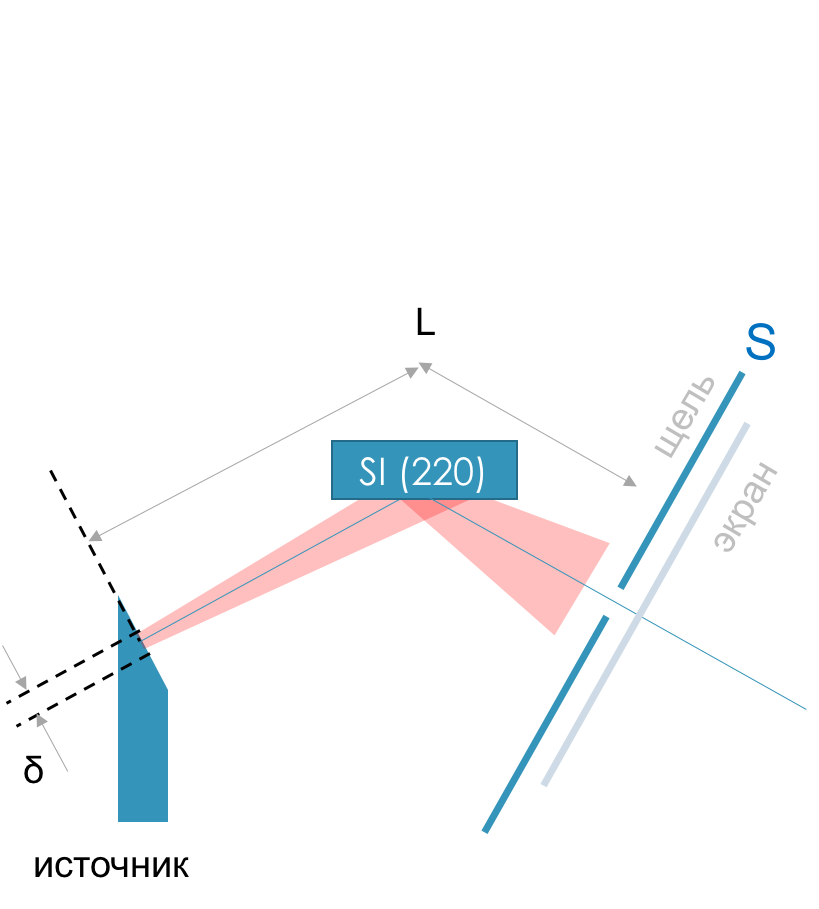
\includegraphics[width=0.45\textwidth]{images/single_crystal_schem.png}\label{ris:single_crystal_schem_lamtet_a}}
  \hfill
  \subfloat[]{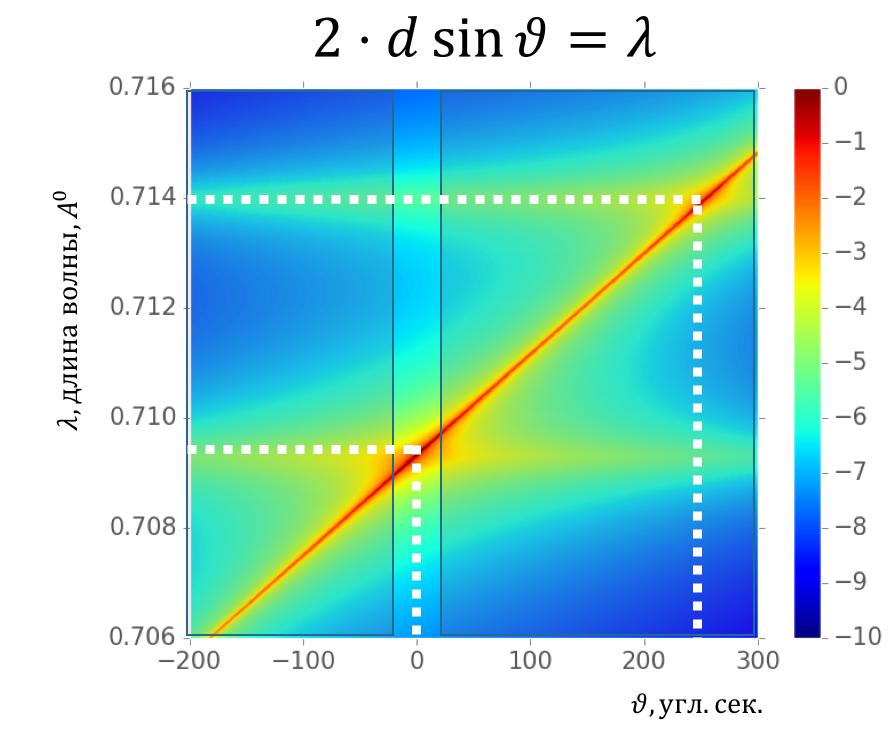
\includegraphics[width=0.45\textwidth]{images/single_crystal_schem_lamtet.png}}

  \caption{(a) Схема однокристального эксперимента. (b) Спектрально угловое распределение после
   отражения расходящегося, полихромотического пучка от кристалла Si(220),
   положение щелевых устройств обозначено синей линией вблизи $\pm 20$ угл.сек.}
  \label{ris:single_crystal_schem_lamtet}
\end{figure}

На рис. \ref{ris:single_crystal_schem_lamtet}, по своей сути, изображен принцип работы монохроматора,
когда после взаимодействия с кристаллом, разные длины волн отражаются под разными углами в
соответсвии с законом Брэгга.

Кривая отражения в однокристальном эксперименте (рис. \ref{ris:single_crystal_schem_lamtet_a}), в котором сканирование осуществляется
 с помощью детектора, жестко связанного с щелевым устройством, линейного размера S, находящегося на расстоянии $L$ от источника, задается следующим образом

\begin{equation} \label{eq:p_single_crystal}
  P_{single}(\theta) = \sum_{\lambda = -\infty}^{\infty}g_{\lambda}(\lambda) \cdot \sum_{\vartheta = \vartheta_{s1}}^{\vartheta_{s2}}
  g_{\vartheta}(\vartheta) P_M(\vartheta - \frac{\lambda - \lambda_1}{\lambda_1}\tan(\theta_B))
 \end{equation}
\noindent
где $\vartheta$ - угол падения излучения на кристалл, в случае не расходящегося пучка $\vartheta = 0$, в
случае, например, синхротронного источника $\vartheta \in (-6^o; 6^o) $; $g_{\lambda}(\lambda)$
- спектральная плотность распределения пучка (\ref{eq:source_spectral}); $g_{\vartheta}(\vartheta)$ - угловая плотность
распределения пучка (\ref{eq:source_angle}); $P_M$ - коэффициент отражения от неподвижного кристалла, далее мы будем его называть монохроматором,
слагаемое $\frac{\lambda - \lambda_1}{\lambda_1}\tan(\theta_B)$ -
возникает из условия Брэгга и говорит о том, что разные длины волн отражаются под разными углами.
 Суммирование проводится, во-первых, вдоль угловой апертуры детектора, которая задается размером
 щелевого коллиматора перед ним, а пределы определяются исходя из ее углового положения $\theta$ относительно
 оптической оси (зеркально отраженного луча) $\vartheta_{s1} = \theta - \frac{S}{2L}$, $\vartheta_{s2} = \theta + \frac{S}{2L}$,
 $S $ - линейный размер щелевого устройства, $L$ - расстояние от источника до щели.
 Во-вторых, суммирование осуществляется по всем $\lambda$, из-за свойства детектора не различать разные длины волн.
На рис. \ref{ris:zero_exp} приведен результат сканирования расходящегося пучка от рентгеновской
трубки после отражения от неподвижного кристалла кремния Si(220) для разных размеров щелевого коллиматора
в сравнении с расчетными.
